\documentclass[12pt, a4paper, oneside]{book}
\usepackage[hidelinks]{hyperref}
\usepackage[english]{babel}
\usepackage[chapter]{algorithm}
\usepackage{graphicx}
\usepackage[utf8]{inputenc}
\usepackage[T1]{fontenc}
\usepackage{setspace}
\usepackage{natbib}
\usepackage{siunitx}
\usepackage{comment}
\usepackage{bm}
\usepackage{amsmath}
\usepackage{enumitem}
\usepackage{subcaption}
\usepackage{lastpage}
\usepackage{fancyhdr}
\usepackage[utf8]{inputenc}
\usepackage[table]{xcolor}
\usepackage{multirow}

\usepackage[utf8]{inputenc}
 
\usepackage{bera}% optional: just to have a nice mono-spaced font
\usepackage{listings}
\usepackage{xcolor}

\usepackage[colorinlistoftodos,prependcaption,textwidth=3.2cm]{todonotes}

\usepackage[left=4cm, right=3cm]{geometry} % aby to vytlacene bolo rozumne posunute vpravo (aby vazba neskodila textu)


\colorlet{punct}{red!60!black}
\definecolor{background}{HTML}{EEEEEE}
\definecolor{delim}{RGB}{20,105,176}
\colorlet{numb}{magenta!60!black}


\lstdefinelanguage{json}{ % formát json (aby vyzeral pekne, dá sa pozmeniť na iné jazyky)
    basicstyle=\normalfont\ttfamily\footnotesize\linespread{0.8},
    numbers=left,
    numberstyle=\scriptsize,
    stepnumber=1,
    numbersep=8pt,
    showstringspaces=false,
    breaklines=true,
    frame=lines,
    showlines=true,
    tabsize=2,
    backgroundcolor=\color{background},
    literate=
     *{0}{{{\color{numb}0}}}{1}
      {1}{{{\color{numb}1}}}{1}
      {2}{{{\color{numb}2}}}{1}
      {3}{{{\color{numb}3}}}{1}
      {4}{{{\color{numb}4}}}{1}
      {5}{{{\color{numb}5}}}{1}
      {6}{{{\color{numb}6}}}{1}
      {7}{{{\color{numb}7}}}{1}
      {8}{{{\color{numb}8}}}{1}
      {9}{{{\color{numb}9}}}{1}
      {:}{{{\color{punct}{:}}}}{1}
      {,}{{{\color{punct}{,}}}}{1}
      {\{}{{{\color{delim}{\{}}}}{1}
      {\}}{{{\color{delim}{\}}}}}{1}
      {[}{{{\color{delim}{[}}}}{1}
      {]}{{{\color{delim}{]}}}}{1},
}

\makeatletter
\def\@makechapterhead#1{% nastavenie názvov kapitol - aby to bol číslovaný názov
  \vspace*{50\p@}
  {\parindent \z@ \raggedright \normalfont
    \interlinepenalty\@M
    \Huge\bfseries  \thechapter.\quad #1\par\nobreak
    \vskip 40\p@
  }}
\makeatother

\setstretch{1.5} % nastavenie veľkosti riadku


\begin{document}

    % bez tychto riadkov sa kazi cislovanie obsahu (ak ma obsah viac ako jednu stranu, tak cisla v obsahu su ok, ale obsah samotny ma blbo cislo strany)
    \pagestyle{fancy}
    \fancyhf{}% Clear page header/footer
    \renewcommand{\headrulewidth}{0pt}% No header rule
    \fancyfoot[C]{\thepage}

    \frontmatter
    \input front_pages/cover.tex
    \input front_pages/title_page.tex
    \input front_pages/assignment.tex
    \input front_pages/affidavit.tex
    \input front_pages/acknowledgment.tex
    \input abstracts/abstract_en.tex
    \input abstracts/abstract_sk.tex
    \tableofcontents
    
    \mainmatter
    \pagestyle{plain}
    
    
    \listoffigures  % zoznam obrazkov
    
    %kapitoly
    \chapter*{Úvod}
\addcontentsline{toc}{chapter}{Úvod}


\todo{Uvod}
    \chapter{Overview}
\label{chap:overview}


\section{Space debris problem}

The rising population of space debris is threat to the satellites. Many non-controlled objects are orbiting the Earth. We need to know the trajectory and position of these objects to minimize possibility of collision with satellites. Cataloguing these objects can help us to prevent unnecessary collisions by moving satellites in advance. \cite{silha2019development}
\section{Existing system}

The Department of Astronomy and Astrophysics
(DAA), Faculty of Mathematics, Physics and Informatics of Comenius University in Bratislava, Slovakia uses a 70 cm Newtonian telescope \ref{fig:telescope} for observation and developed system for tracking space debris and other objects.

Object catalogization consists of these steps \cite{krajvcovivc2019selected}:
\begin{enumerate}
    \item Star field identification\\
    Star field is identification with Astrometry.NET scripts
    \item Image reduction\\ 
    Removing multiplicative errors from the image caused by imperfect circumstances. These errors are removed by subtracting \textit{bias} frame (taken with closed shutter).
    \item Background estimation and subtraction\\
    Sigma clipping is used to estimate and subtract background from the image
    \item Objects search and centroiding (segmentation)\\
    Object are detected in the image and their position and other attributes are saved in text file.
    \item Astrometric reduction\\
    Position of the object from previous step is translated to the equatorial coordinates.
    \item Masking\\
    Masking is used to remove duplicate and stationary objects
    \item Tracklet building\\
    Finding trajectory of moving objects
    \item Object identification\\
    Identification of the object in the catalogue

\end{enumerate}

\begin{figure}[h!]
    \centering
    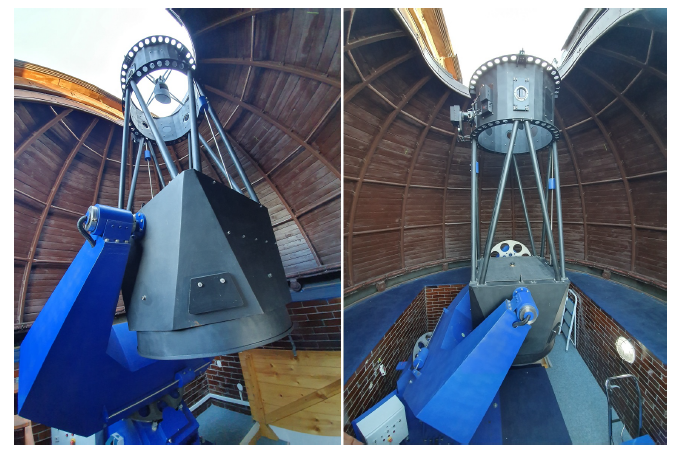
\includegraphics[width=60mm]{chapters/images/telescope.PNG}
    \caption{Telescope}
    \label{fig:telescope}
\end{figure}


\subsection{Tracklet building}

I am focused on tracklet building in my thesis. Tracklet is a data structure containing consecutive observations of a frame object in time. We can refer to tracklet as trajectory of the object. 

\begin{figure}[h!]
    \centering
    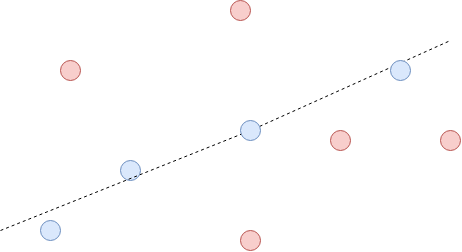
\includegraphics[width=100mm]{chapters/images/trajectory_img.png}
    \caption{Trajectory and tracklet of object}
    \label{fig:TB_trajectory}
\end{figure}

Blue object in the figure \ref{fig:TB_trajectory} are representing tracklet and red object are points which were not chosen to tracklet. We can then approximate this positions by imaginary line which represents trajectory of object in time and space.

We can approximate object trajectory by line as we are observing only small part of sky where true trajectories of object in Earth orbit are very close to simple line. 

In this system, Simple linear regression (SLR)  is used to find sequence of object on a line \cite{krajvcovivc2019selected}. Tracklet building is then realized in following steps:
\begin{enumerate}
    \item Creating Cartesian product of objects from first and second frame
    \item Computing angular velocity and position angle of two point for every couple
    \item For each k-tuple we check if exists object in the next frame with position close to computed next position from previous step. This object is added to tracklet.
    \item Line parameters for k-tuples are updated with SLR
    \item Continue iteratively on step 3
\end{enumerate}

After processing object from all frames tracklets are saved to text file. 


\subsection{Equatorial coordinate system}

Position of object after \textit{Astrometric reduction} is given in Equatorial coordinates. Equatorial coordinates represents position  of object on celestial sphere \cite{thompson2006coordinate} . 

\begin{figure}[!h]
    \centering
    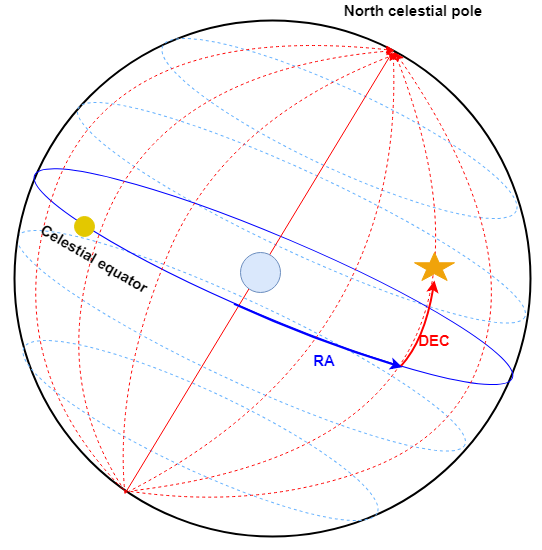
\includegraphics[width=100mm]{chapters/images/equatorial_coordinates.png}
    \caption{Equatorial coordinates of object}
    \label{fig:Equatorial_coordinates}
\end{figure}

Position consists of two coordinates. 
\begin{itemize}
    \item \textbf{Declination} - measures the angular distance from celestial equator. Declination has values from $-90°$ up to $+90°$. $-90°$ value represents South pole and $+90°$ the North pole.
    \item \textbf{Right ascension} - measures angular distance from Greenwich meridian along celestial equator. Right ascension is usually measured in sidereal hours from $0$ hour $0 min$ $0$ sec to $24$ hour. For easier manipulation can be rewritten as angle.
\end{itemize}

Position of object in equatorial or heliographic coordinates are computed in astrometric reduction with use of information from FITs header (FITs images are made by telescope).

Although equatorial coordinates do not represent position on 2-D plane, as our filed of observation is very small we can assume that Equatorial coordinates behaves such as Euclidean coordinates. 

\section{Deep Learning}

In this section I am referencing information from the book \textit{Deep Learning} \cite{Goodfellow-et-al-2016} chapters 1 and 10.
\\
Computers are good in solving problems which can be described formally by mathematical rules. There are problems easy for humans but hard to be formally described.  With lots of training data system can gather knowledge from experience without the need for human to specify all needed concepts. System is building a hierarchical graph of concepts which enables him to learn complicated concepts from similar ones. Cause this graph of concepts is very deep we call this approach \textbf{Deep Learning}.

\subsection{Recurrent neural network}

Recurrent neural networks (RRNs) are family of neural networks specialized for processing sequential data. RNNs are made to process sequences of values $ x^{(1)}, x^{(2)},x^{(3)}, ..., x^{(n)} $. They can process long sequences and most of recurrent networks can work also with sequences with variable length. 

For processing sequences of fixed length we can use simple multi-layer perceptron model, however this model is not able to efficiently learn  dependencies between inputs. For example in language word order might not change the meaning of sentence. 
\begin{center}
    \textbf{In last year, there were Covid pandemic.}\\
    \textbf{There were Covid pandemic last year.}
\end{center}
Meaning of both sequences is the same but the target words \textit{Covid pandemic} are not in the same place in these sentences. We want from network to accumulate knowledge from previous input words in processing of next word. In RNNs same function of previous output and current input is used for each input. This process stores information from previous time point in so called \textbf{hidden state} $h^{(t)}$. We can better imagine this process by unfolding neural network in time.

\begin{figure}[!h]
    \centering
    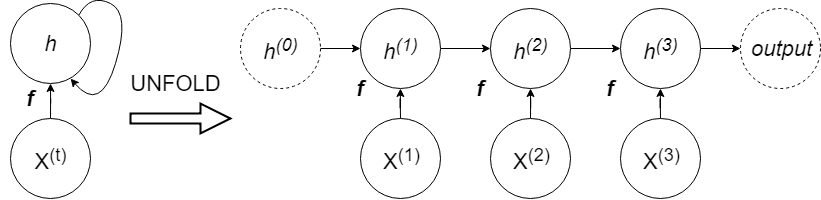
\includegraphics[width=140mm]{chapters/images/RNN_unfold.png}
    \caption{Recurrent neural network processing information of length 3}
    \label{fig:Unfold}
\end{figure}

Each node in unfolded graph represents one time instance. We can rewrite one step computation
$$ h^{(t)} = f(h^{(t-1)}, x^{(t-1)}, \Theta)$$

It is proven that any function computable by a Turing machine can be computed by RNN of a finite size.

\subsubsection{Leaky recurrent neural network}

Problem with big RNN is vanishing or exploding gradient. Unfolded graph of RNN acts like multi-layer perceptron. If sequences are long our imaginary network is very deep. In backward pass is likely that gradient will vanish to have absolutely zero effect on previous inputs, or explode and focus only on one example. Leaky RNNs have lateral connections in time to avoid this effect (figure \ref{fig:RNN_lateral}). They accumulate information over long time.  

\begin{figure}[!h]
    \centering
    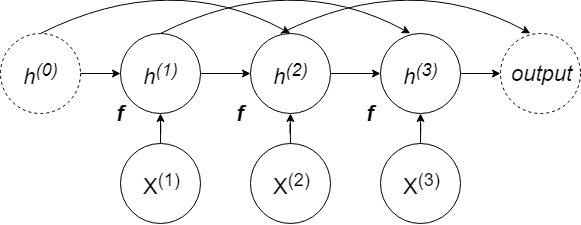
\includegraphics[width=140mm]{chapters/images/RNN_leaky.png}
    \caption{Recurrent neural network with lateral connections every second time instance }
    \label{fig:RNN_lateral}
\end{figure}

\subsection{Long short term memory - LSTM}

Leaky RNN accumulate information over long period of time. However in some cases we want to forget part of information we learned, for example if our sequence consists of subsequences. This problem was solved by introducing gated units like \textbf{LSTM}. Gated unit use gates - learnable parameters which controls amount of information passing through. 


\begin{figure}[!h]
    \centering
    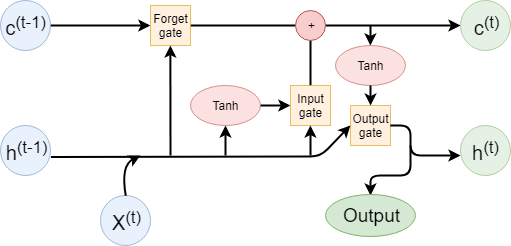
\includegraphics[width=140mm]{chapters/images/LSTM.png}
    \caption{LSTM unit}
    \label{fig:LSTM}
\end{figure}

LSTM has three two states. 
\begin{itemize}
    \item $c^{(t)}$ represents \textbf{cell state} - cell state is a path for information to run down through whole network like lateral connections in leaky units
    \item $h^{(t)}$ represents \textbf{hidden state} - hidden state is previous output of LSTM.
\end{itemize}

LSTM also have three gates: Input, output and forget gate. Each gate is a pointwise multiplication of first input and output of nonlinear function from second input (fig. \ref{fig:LSTM_gate}). Gate has two weight matrices $U$ for input vector and $W$ for hidden state vector.


\begin{figure}[!h]
    \centering
    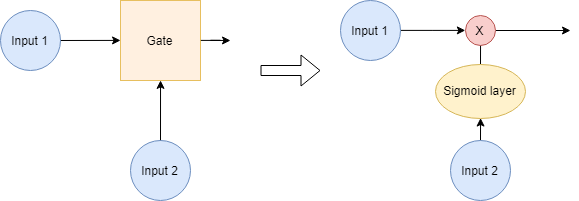
\includegraphics[width=120mm]{chapters/images/LSTM_gate.png}
    \caption{Gate}
    \label{fig:LSTM_gate}
\end{figure}

Input $x^{(t)}$ is at first concatenated with hidden state $h^{(t-1)}$ and with $c^{(t-1)}$ goes through Forget gate. Let $f^{(t)}$ be the output from sigmoid layer from the gate.

\begin{eqnarray}
    f^{(t)} = \sigma \left(  bias^f + \sum_j U^f_{i,j} x^{(t)}_j + \sum_j W^f_{i,j} h^{(t-1)}_j \right)
\end{eqnarray}

Next cell state is then computed:


\begin{eqnarray}
    I^{(t)} = \sigma \left(  bias^I + \sum_j U^I_{i,j} x^{(t)}_j + \sum_j W^I_{i,j} h^{(t-1)}_j \right) \\
    l^{(t)} = tanh \left(  bias^l + \sum_j U^l_{i,j} x^{(t)}_j + \sum_j W^l_{i,j} h^{(t-1)}_j \right) \\
    c^{(t)} = f^{(t)}c^{(t-1)} + I^{(t)}l^{(t)}
\end{eqnarray}

where $I^{(t)}l^{(t)}$ is output of input gate and $l^{(t)}$ is LSTM internal unit.

Next hidden state is computed 
\begin{eqnarray}
    O^{(t)} = \sigma \left(  bias^O + \sum_j U^O_{i,j} x^{(t)}_j + \sum_j W^O_{i,j} h^{(t-1)}_j \right) \\
    h^{(t)} = tanh(c^{(t)}) O^{(t)}
\end{eqnarray}

Let $n$ be the size of input vector and $m$ size of hidden state vector. At the end LSTM unit consists of four pairs of matrices - $W$ with shape $m \times m$ and $U$ with shape $m \times n$. Total number of trainable parameters is then 
\begin{equation}
N = 4 \cdot ( n \times m ) 
\end{equation}

LSTM network have been shown to learn long-term dependencies more easily than the simpler recurrent neural networks. LSTM are good for forecasting time series. Input for the system is some subsequence of time series and output is next point in time series.  

One disadvantage of LSTM is length of training. Using time folding with this many parameters cause long training of LSTM even with relatively low input and hidden dimensions.

\section{PyTorch}

Pytorch is an open source machine learning framework developed by Facebook \cite{PytotchDocumentation}. In this section I am referencing resources \cite{Pytorch} and \cite{PytotchDocumentation}. 

Pytorch is Python framework which allows to write model in easy to read idiomatic Python. Due easy debugging and clear syntax, Pytorch has been used by research communities and is very good as introduction to deep learning. Pytorch provide accelerated computations using GPUs, which can be $50 \times$ faster than same operations computer on CPU.

\subsection{Autograd}

Autograd is component in Pytorch which is responsible for automatic computation of gradient. PyTorch \textit{tensor} is able to remember all operations performed on him. Autograd can computer derivatives of this operations with respect to their inputs. 

This is essential for computing gradients in backpropagation algorithm in deep neural networks where analytic solutions for gradients are very complex.

\begin{lstlisting}[language=Python]
>>> import torch
>>> x = torch.tensor([5.], requires_grad=True)
>>> z = x**2
>>> z
tensor([25.], grad_fn=<PowBackward0>)
>>> x.grad
None
>>> z.backward()  # calling of autograd
>>> x.grad
tensor([10.])
\end{lstlisting}

As we can see in code example we are computing derivative of function $f(x) = x^2$ with respect to $x$. We can confirm that derivative $\frac{d x^2}{d x} = 10$

$$ \frac{d x^2}{d x} = 2x = 2\cdot 5 = 10 $$

Every \textit{tensor} has \textit{grad} attribute which is filled after call of autograd. If option \textit{requires\_grad} is set to \textit{True} gradients are computes with respect to this variable.

\subsection{Neural network model}

In Pytorch we define neural network model as Python class derived from \textit{nn.Model} class. Class must implement these methods
\begin{enumerate}
    \item \textbf{\_\_init\_\_} - in this function we define our layers
    \item \textbf{forward} - this function implement forward pass of our network.
\end{enumerate}

\begin{lstlisting}[language=Python]
class SimpleNet(nn.Module):
    def __init__(self):
        super(SimpleNet, self).__init__()
        self.l1 = nn.Linear(10,2)
    
    def forward(self, x):
        y = self.l1(x)
        return torch.tanh(y)
\end{lstlisting}


This is all we need for our simple network. Backpropagation in the training is made by Optimizer from package \textit{torch.optim}.

    \chapter{Goal of thesis}





\todo[inline, color=red!70]{Ciel prace}
    \chapter{Software design}


\todo[inline, color=red!70]{Software design}
    \chapter{Propose methods}

\section{Data generator}

Machine learning models need a fair amount of data examples for training. In supervised learning, each training example consists of input data and target value. In out case input data point is series of pictures captured by telescope and target value is tracklet of object. Not many of these pairs picture series, tracklet are available for training. If we want to train Deep neural network we need to make artificial training data.

\subsection{starGen.r}

The Department of Astronomy and Astrophysics has provided existing solution for this problem. \textbf{StarGen} script is written in language R and is capable of generating single FITS image. It has adjustable parameters:
\begin{itemize}
    \item \textbf{dimX, dimY} - representing size of image
    \item \textbf{starCount} - number of generated stars
    \item \textbf{fwhm} - full width at half maximum (size of star)
    \item \textbf{briMin, briMax} - brightness parameters
    \item \textbf{method} - method used for star generation, gauss, cauchy, line
\end{itemize}

Script is able to generate FITS images with set number of stars. Stars can be seen as point light source or line which simulates telescope movement. 


\begin{figure}[!h]
\centering
\begin{subfigure}{.5\textwidth}
  \centering
  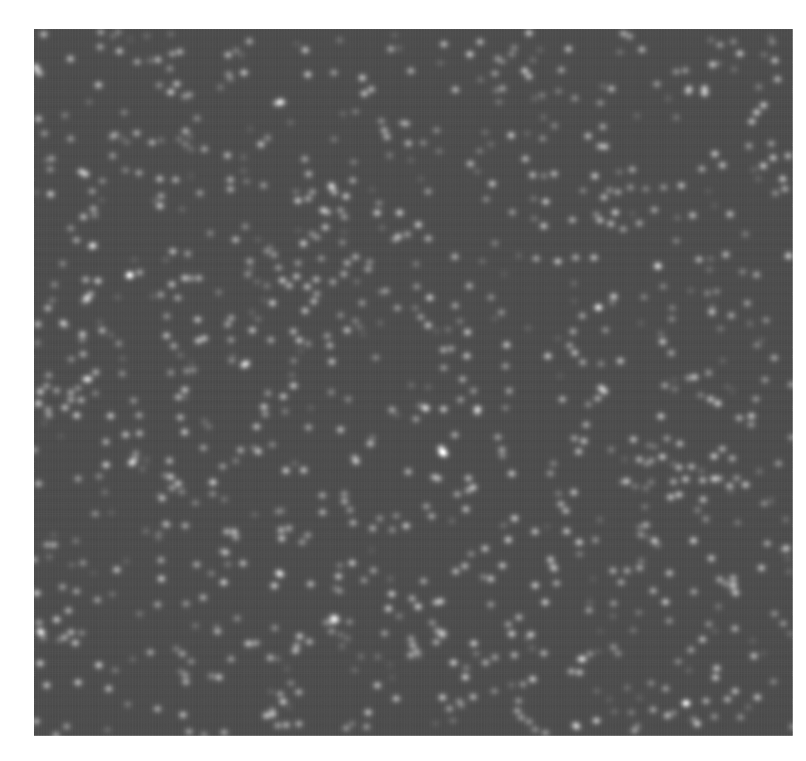
\includegraphics[width=1.0\linewidth]{front_pages/images/original_star_gen.png}
  \caption{Image with 1000 stars and fwhm 10}
  \label{fig:star_gen_orig}
\end{subfigure}%
\begin{subfigure}{.5\textwidth}
  \centering
  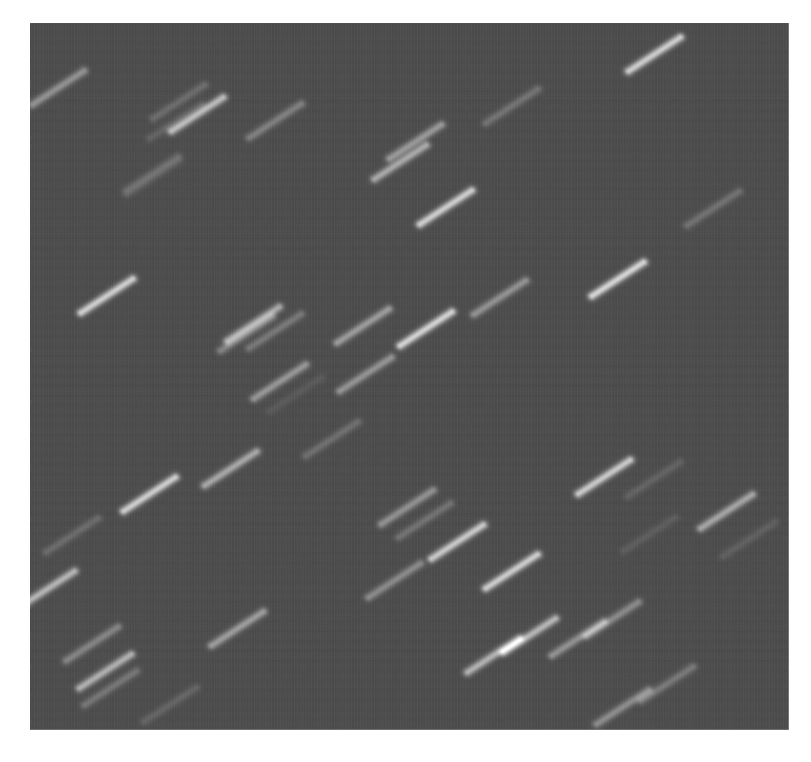
\includegraphics[width=1.0\linewidth]{front_pages/images/original_star_gen_lines.png}
  \caption{Image with lines, 10 fwhm, 50 stars }
  \label{fig:star_gen_orig_lines}
\end{subfigure}
\caption{Images generated by starGen.r}
\label{fig:star_gen}
\end{figure}

\subsection{StarGen.py}

\textit{starGen.r} generates images which cant be directly used as training examples for machine learning models. Whole script was rewritten to Python and modified. 

\begin{itemize}
    \item \textbf{Series of images} \\
    For training data we need series of images not only one image. New generator generates image series of length 8.
    
    \begin{figure}[!h]
    \centering
    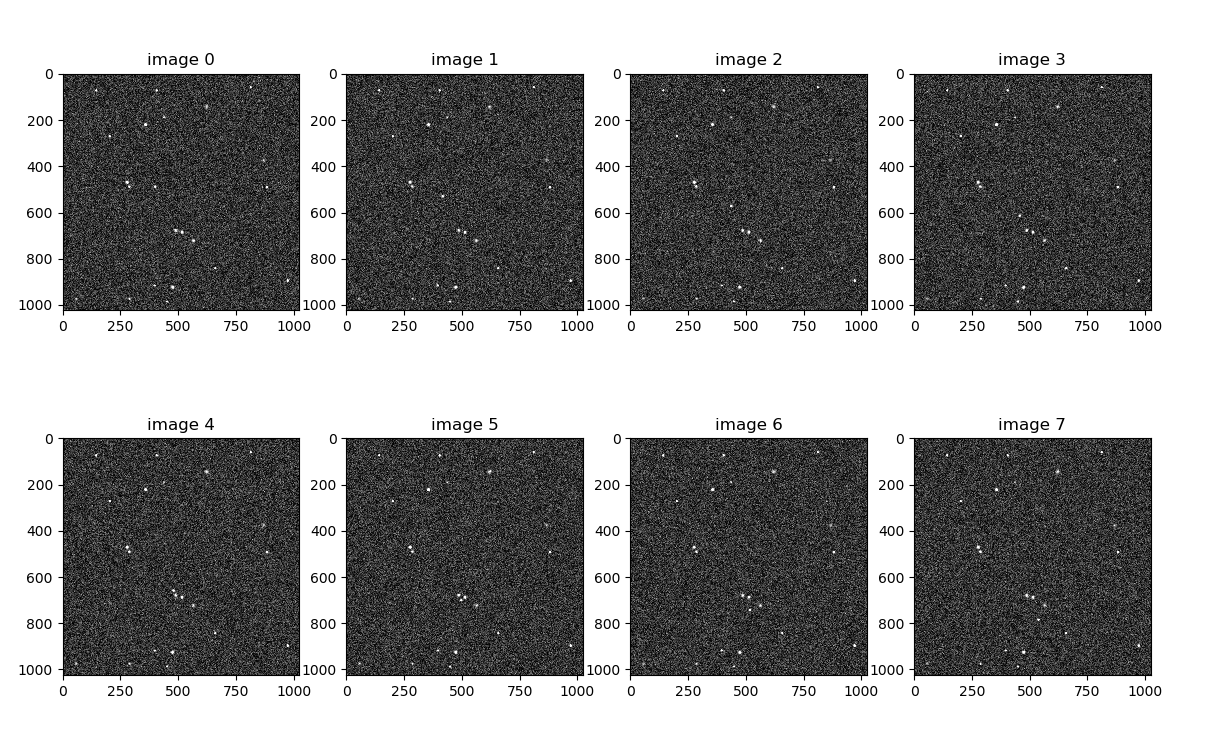
\includegraphics[width=150mm]{chapters/images/data_series.PNG}
    \caption{Series of 8 images created by generator}
    \label{fig:series_data_generator}
    \end{figure}
    
    \item \textbf{Objects}\\
    Original script is not producing tracking object in the picture. We have modified script to produce variable number of objects and their trajectories. Trajectory consists of object positions in each image of the series.
    
    \begin{figure}[!h]
    \centering
    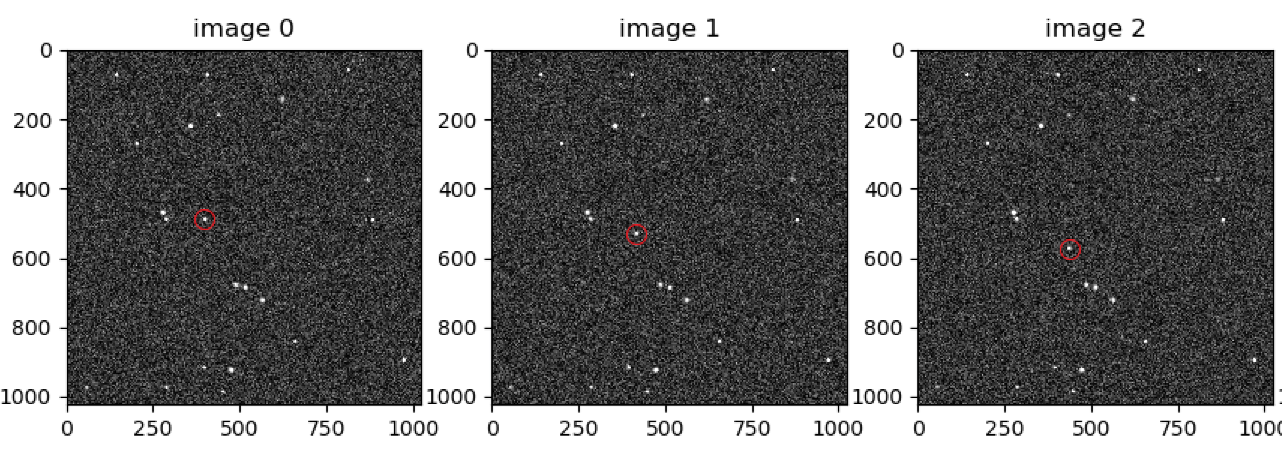
\includegraphics[width=1.0\linewidth]{chapters/images/cast_seria_object_vyznaceny.PNG}
    \caption{Moving object in images}
    \label{fig:object_data_generator}
    \end{figure}
    
    \item \textbf{TSV output file}\\
    Positions of both stars and object in each frame are stored to \textit{.tsv} file with same structure as after \textbf{Segmentation} step in existing system \ref{chap:overview}. This ensures that artificial data will be compatible with real data.
    Files contains one extra Boolean field for marking object position.
    
    
    \begin{figure}[!h]
    \centering
    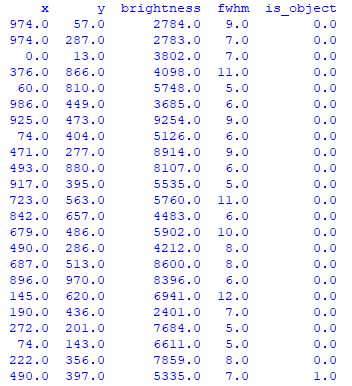
\includegraphics[height=100mm]{chapters/images/tsv_file.PNG}
    \caption{Tsv file representing positions of stars and objects}
    \label{fig:tsv_file_data_generator}
    \end{figure}
    
    \item \textbf{Point objects}\\
    For training purposes and simplicity, script is generating only point light sources.
    
\end{itemize}

Parameters for script are stored in \textit{config.yml} file. We can set: number of series, number of objects and stars in frame, stars and object paramaters. Script produce set number of series consisting of eight FITS images and eight .tsv files.






 




\section{SVM method}

Support-vector machine (SVM) model is supervised machine learning model used for classification. It projects original data point into higher dimension and perform maximal-margin classification in this higher dimension space. 

\todo[inline, color=yellow]{zdroj na svm}

We can use this property and train SVM to classify input tuples of size $k$ to two classes
\begin{enumerate}
    \item \textbf{On line}\\
    This class represents k size ordered tuples with their point laying on the line with same distances between points in tuple. Each two adjacent points in tuple have to be equally distant and  lay on the same straight line.
    
    \item \textbf{Not on line}\\
    This class represents k size tuples which are not \textit{on line}
\end{enumerate}

\begin{figure}[!h]
\centering
\begin{subfigure}{.4\textwidth}
  \centering
  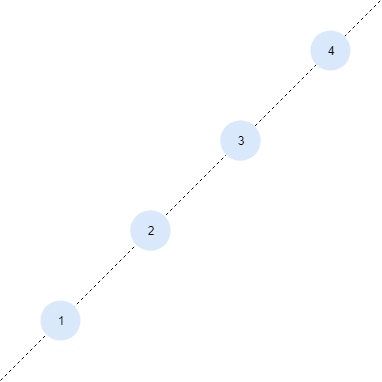
\includegraphics[width=1.0\linewidth]{chapters/images/svm_class1.PNG}
  \caption{On line class example}
  \label{fig:svm_class2}
\end{subfigure}%
\begin{subfigure}{.37\textwidth}
  \centering
  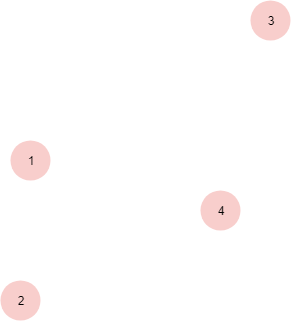
\includegraphics[width=1.0\linewidth]{chapters/images/svm_class2.PNG}
  \caption{Not on line class example }
  \label{fig:svm_class1}
\end{subfigure}
\caption{SVM classification classes}
\label{fig:svm_classes}
\end{figure}

\subsection{Algorithm}

\begin{figure}[!h]
    \centering
    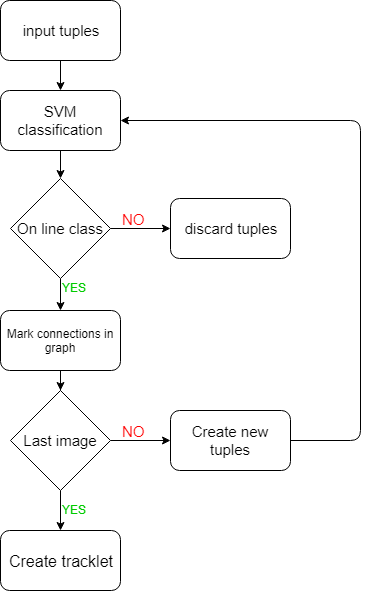
\includegraphics[height=12cm]{chapters/images/SVM_activity_diagram2.PNG}
    \caption{SVM method activity diagram}
    \label{fig:svm_activity_diagram}
\end{figure}

\textbf{Input tuple} consist of $k$ positions $[x, y]$. First position of object in tuple is position of an object from $i$-th image's .tsv file, second from $(i+1)$-th image's file and so on. Last position in tuple is from $(i+k)$-th image's .tsv file. Initially tuples are created by applying Cartesian product between positions of objects from first $k$ images. This process will create $n^k$ tuples if $n$ is number of positions in one image 

Tuple is classified with \textbf{SVM classifier} to one of two classes:
On line class, not on line class. \textbf{Not on line} class tuples are discarded and further proceed only \textbf{on line} class tuples

If result of classifier is \textit{On line}, connections between positions in tuple are marked in graph. 

If tuple last element is not position from last image, \textbf{new tuples are created}. First element is removed from tuple, and at the end one position from next image is appended. New tuple will be created for every position from last image.

After processing all input tuples, we find path from position from first image to some position from last image. If such path exists we consider it as \textbf{tracklet} Positions on the path are positions of moving object.

\begin{figure}[!h]
    \centering
    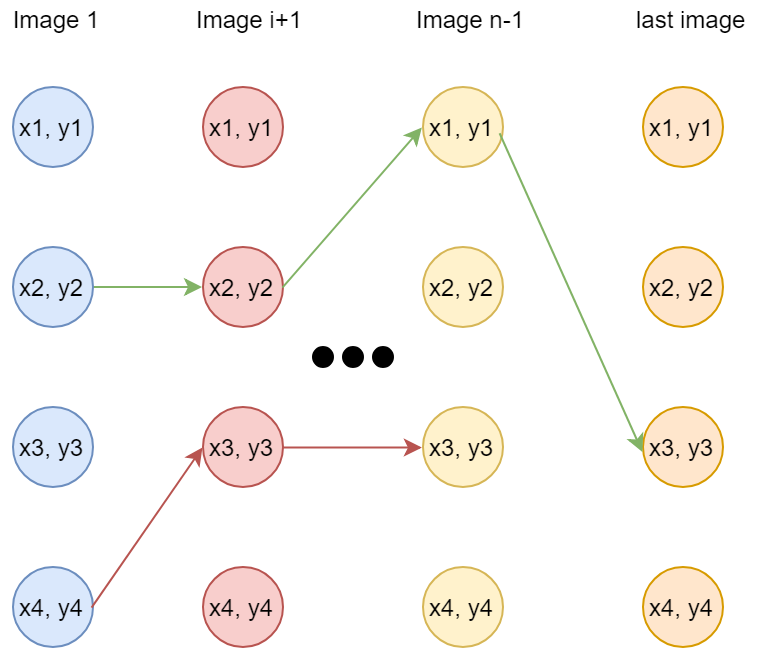
\includegraphics[width=0.8\linewidth]{chapters/images/SVM_graph.PNG}
    \caption{Possible connections in final graph after processing images}
    \label{fig:svm_result_graph}
\end{figure}

In figure \ref{fig:svm_result_graph} there are two possible paths. Green one leads from first image to last image therefore can be declared as tracklet. Nodes in graph are position of moving object in tracklet. Red path is "incomplete", does not lead to last image. 

\subsection{Disadvantages}

Finding moving objects using SVM method turns out not to be reliable. This method is very simple but it comes with a cost.


\subsubsection{Parameter k and creation of input tuples}
Parameter $k$ stays for size of input tuples to SVM classification. Smaller value than $k=3$ cannot be used, because for smaller values all tuples would fulfill the condition for On line class. As value of $k$ is higher classification is more precise. Yet, high value of $k$ leads to high number of input tuples. Let $n$ be number of positions in one image, then $n^k$ is number of input tuples. Value of $n$ can be in hundreds so computation becomes very slow for even slightly higher values of $k$ such as $4$ or $5$.    

\subsubsection{Big number of Not on line class in real data}
SVM classification trained on $50$ thousand tuples with size $k=3$ has had above $96\%$ accuracy. Only $ 3\% $ of validation data were classified as False negative.  


\begin{center}
\begin{table}[!h]
\renewcommand{\arraystretch}{2}
\begin{tabular}{ p{2cm} p{3cm} p{5cm} p{3cm} | } 
\cline{3-4}
& & \multicolumn{2}{|c|}{True class}\\
\cline{3-4}
 &  & \multicolumn{1}{|l|}{\textbf{On Line}}& \multicolumn{1}{|l|}{\textbf{Not On Line}} \\
\hline
\multicolumn{1}{|l|}{\multirow{2}{4em}{Predicted class}} & \multicolumn{1}{|l|}{\textbf{On Line}} & \multicolumn{1}{|l|}{4996}  & \multicolumn{1}{|l|}{4} \\
\cline{2-4}
\multicolumn{1}{|l|}{} & \multicolumn{1}{|l|}{\textbf{Not On Line}} & \multicolumn{1}{|l|}{363}  & \multicolumn{1}{|l|}{4637}  \\
\hline
\end{tabular}
\renewcommand{\arraystretch}{1}
\caption{Confusion Matrix for 10 000 examples, k=3}
\label{tab:svm_conf_matrix}
\end{table}
\end{center}

In real world data, if only one moving object is in the images, every input tuple except one containing positions of moving object belongs to not on line class. This disproportion between classes leads to big number of false negative. In result, we classify many tuples as on line class, but only one truly belongs to that class. 

If our algorithm classify more than one tuple from last generation (tuples with last element from last image) as on line class we can certainly say that in our graph exists at least that many paths from first image to last image. Real number of paths can be much larger.

In testing scenario with $k=3$, there were 180 tuples from last generation classified as on line class. That means that me have identified at least 179 bad tracklets. With higher $k=4$ results were similar. Algorithm identified at least 143 bad tracklets, even classification had $98\%$ accuracy. 

\begin{center}
\begin{table}[!h]
\renewcommand{\arraystretch}{2}
\begin{tabular}{ p{2cm} p{3cm} p{5cm} p{3cm} | } 
\cline{3-4}
& & \multicolumn{2}{|c|}{True class}\\
\cline{3-4}
 &  & \multicolumn{1}{|l|}{\textbf{On Line}}& \multicolumn{1}{|l|}{\textbf{Not On Line}} \\
\hline
\multicolumn{1}{|l|}{\multirow{2}{4em}{Predicted class}} & \multicolumn{1}{|l|}{\textbf{On Line}} & \multicolumn{1}{|l|}{4997}  & \multicolumn{1}{|l|}{3} \\
\cline{2-4}
\multicolumn{1}{|l|}{} & \multicolumn{1}{|l|}{\textbf{Not On Line}} & \multicolumn{1}{|l|}{152}  & \multicolumn{1}{|l|}{4848}  \\
\hline
\end{tabular}
\renewcommand{\arraystretch}{1}
\caption{Confusion Matrix for 10 000 examples, k=4}
\label{tab:svm_conf_matrix2}
\end{table}
\end{center}

With so many false negative examples we cannot detect true moving object. Due to these problems SVM method was rejected.

    





\todo[inline, color=red!70]{Pouzite metody}
    \chapter{Research}

\todo[inline, color=red!70]{Vyskum}
    \chapter{Results}

\todo[inline, color=red!70]{Vysledky na datach}
    \chapter*{Conclusion}
\addcontentsline{toc}{chapter}{Conclusion}

\todo[inline, color=green!60]{Conclusion}

\medskip

\bigskip


    
    \appendix
    \chapter{Prílohy}
\label{appendix_files}

\todo[inline, color=red!70]{Prílohy}


    
    \backmatter
    \nocite{*}
    \bibliographystyle{unsrt}
    \bibliography{references}
    
    \listoftodos[TODOs:] % sem sa automaticky spisu tvoje TODOs aby si to mal pocas pisania prehladne

\end{document}